% Chapter 1

\chapter{Groups growth model} % Main chapter title

\section{Introduction}

Social groups, informal or formal, are building mesoscopic elements of every socio-economic system. Their emergence, evolution, and disappearance are at the heart of change in a social system \cite{}. Settlements, villages, towns and cities are formal and highly structured social groups of countries. Their organisation and growth determine the functioning and sustainability of every society \cite{barthelemy2016structure}. Companies are the building blocks of every economy and their dynamics are important indicators of level of development of every economy \cite{hidalgo2009building}. Scientific conferences, as a scientific groups, enable fast dissemination of the latest results, exchange and evaluation of ideas as well as a knowledge extension, and thus are integral part of science \cite{smiljanic2016theoretical}. The membership of individuals in various social groups, online and offline, can be essential when it comes to quality of their life \cite{montazeri2001anxiety, davison2000talks, cho2012tea}. Therefore, it is not surprising that the social group dynamics and their sustainability are at the center of the attention of many researchers \cite{aral2012identifying,gonzalez2013broadcasters, torok2013opinions, yasseri2012dynamics}.\\

The abundance of data enabled the application of methods and paradigms from statistical physics in studying the structure and dynamics of social systems \cite{castellano2009statistical}. The main argument for using statistical physics to study social systems is that they consist of a large number of interacting individuals. Due to this, they exhibit different patterns in their structure and dynamics, commonly known as \textit{collective behavior}. A collective behavior, observed both in physical and social systems, is enforced by a few basic properties of building units and is independent of all other characteristics. The phenomenon is known as \textit{universality} in physics and is commonly observed in social systems such as in voting behavior \cite{chatterjee2013universality}, or scientific citations \cite{radicchi2008universality}. The discovery of universality and scaling in phenomena indicate the existence of universal and straightforward mechanisms that govern the dynamics of a system \cite{}.\\  


The availability of large-scale and long-term data on various online social groups has enabled the detailed empirical study of their dynamics. The focus was mainly on the individual groups and how structural features of social interaction influence whether individuals will join the group \cite{backstrom2006group} and remain its active members \cite{smiljanic2016theoretical, smiljanic2017associative}. The study on LiveJournal \cite{backstrom2006group} groups has shown that decision of an individual to join a social group is greatly influenced by the number of her friends in the group and the structure of their interactions. The conference attendance of scientists is mainly influenced by their connections with other scientists and their sense of belonging \cite{smiljanic2016theoretical}. The sense of belonging of an individual in social groups is achieved through two main mechanisms \cite{smiljanic2017associative}: expanding of the social circle at the beginning of joining the group and strengthening of the existing connections in the later phase. The dynamics of social groups depend on their size \cite{}. Analysis of the evolution of large-scale social networks has shown that edge locality plays a critical role in the evolution of social networks \cite{leskovec2008microscopic}. Small groups are more cohesive with constant membership, while large groups tend to change their active members constantly \cite{PNAS}. Previous research focused on the growth of the single group, the evolution of its social network, and the influence of the structure on its growth. However, how growth mechanisms influence the distribution of members of one social system among groups is still anecdotal.\\

Furthermore, it is not clear whether the growth mechanisms of social groups are universal or system-specific. The size distribution of social groups has not been studied in great detail. Rare empirical evidence of size distribution of groups and communities indicates that it follows power-law behavior \cite{}.  The distribution of the size of the cities and firms has been studied in great detail. Analysis of the sizes of the cities shows that the distribution of all cities follows a log-normal distribution, while the distribution of the largest cities resembles Zipf's distribution \cite{fazio2015pareto}. The scaling behavior was observed in the growth of the companies \cite{stanley1996scaling}, while empirical evidence shows that distribution of company sizes follows log-normal behavior and remains stable over decades \cite{amaral1997scaling}. 

Can we create a unique yet relatively simple microscopic model that will reproduce the distribution of members between groups and explain the differences observed between social systems? French economist Gibrat proposed a simple growth model to reproduce companies' and cities' observed log-normal size distribution. However, the analysis of the growth rate of the companies \cite{amaral1997scaling} has shown that growth mechanisms are different from ones assumed by Gibrat. Analysis of the growth of three online social networks showed that population growth is not determined by the population size and spatial factors, and it deviates from Gibrat's law \cite{zhu2014online}. The growth through diffusion and growth by other means have been used as mechanisms in the model used for prediction of rapid group growth \cite{kairam2012life}. The growth mechanisms of various social groups and the source of the scaling observed in socio-economic systems thus remain hidden.\\

Here we analyze the distribution of formal social groups in two different systems: Meetup online platform and subreddits in the Reddit community. We analyze the scaling behavior of size distributions and distribution of growth rates. Analysis of the dependence of growth rates indicates that growth can not be explained through Gibrat's model. We propose a simple microscopic model that incorporates some of the results of previous research \cite{backstrom2006group}. In our model, the social system grows by adding a constant number of new individuals. The number of groups grows as well, and they overlap in terms of membership, i.e., one individual may be a member of more than one group. An individual can create a new group or join an existing one according to some probability. The choice of the existing group depends on the number of social connections already present. We show that the model can reproduce size distributions and growth rate distribution for both studied systems. We analyze the model and show that it can produce a broad set of distributions depending on the value of model parameters.\\

The paper is organized as follows: in Section \ref{sec:data} we describe the data, while in Section \ref{sec:emp} we present our empirical results. In Section \ref{sec:model} we introduce model parameter and rules. Section \ref{sec:results} we demonstrate that model can reproduce the growth of social groups in both systems and show the results for different values of model parameters. Finally, in Section \ref{sec:con}, we present concluding remarks and discuss our results. 


\section{Data \label{sec:data}}
We analyse the growth of social groups from two widely used online platforms: Reddit and Meetup. Reddit \footnote{https://www.reddit.com/} enables sharing diverse web content, while Meetup \cite{www.meetup.com} allows people to use online tools to organize offline meetings. Reddit users interact exclusively online through posts and comments. The building elements of the Meetup community are topic-focused groups, such as food lovers or ICT and data science professionals. Due to their specific activity patterns - events where members meet face-to-face - Meetup groups are geographically localised. 

We compiled the Reddit data from https://pushshift.io/. This site collects data daily and, for each month, publishes merged comments and submissions in the form of JSON files. 
Specifically, we focus on subreddits - social groups of Reddit members interested in a specific topic. We select all subreddits active in 2012 and follow their growth from their beginning until 2017. The considered dataset contains 17000 subreddits, with the oldest originating from 2003 and the youngest being from 2017.\\
For each post under a subreddit, we extracted the information about the user-id of the post owner, subreddit-id, and timestamp. We observed the data from $2006$ to the $2017$ year, and for each subreddit and user-id, we selected timestamp when a user made a post for the first time. For our analysis, we chose subreddits still active in $2017$ while removing small subreddits active for less than a month. The resulting dataset contains $304 007$ subreddits and  $36 595 134$ users. \\
For simulation, we extracted data until $2011-12$ and removed all subreddits with a small amount of activity. This reduced the dataset significantly - we obtained only $17 073$ subreddits with $2 195 677$ active users. 

The Meetup data were downloaded in $2018$ using public API. The Meetup platform was launched in 2003, and at the moment we accessed the data, there were more than 240000 active groups. For each group, we extracted information about the date it had been founded, its location, and the total number of members. We focused on the groups founded from $2003$ until $2017$ in big cities such as London and New York, where Meetup platform achieved considerable popularity. We considered groups active at least one month. There were 4673 groups with $831685$ members in London and 4752 groups with $1059632$ members in New York. In addition, we extracted the Id of each member in the group, which allowed us to obtain complementary information about the date a member joined a group. 

From collected data, for each group, we can calculate the number of new members per month and so the group sizes $S_i$ at each time step (month). The growth rate $R_i$ at step $i$ is obtained as logarithm of successive sizes $R = log(S_t/S_{t-1})$. 

%We select two locations, London and New York, and study the formation and growth of groups in these two locations from 2003 until 2017. The total number of groups studied for London is 4000 and 8000 for New York. 
%Potreban je slican opis za Meetup podatke

While these two communities differ in means of communication between their users and activities these users engage in, there are certain common properties that enable us to use same methods to study the growth of these groups and make comparative analysis of their growth. In both communities, users can create new groups and join existing ones. One user can be a member of more than one group/subreddit and there are no limits in the number of groups. For each meetup group we have an information on when an user has joined the group, i.e., we have an information about the group size at every moments. For a subreddit we have a detailed information about users' activity and this we have an information when a user made a first post. This moment is considered as the moment when the user has joined the subreddit and became an active member. In our case we do not consider activity of when a user leaves the group of subreddit, since this kind of information is not available to us. For these reasons, the size of groups we are considering is non-decreasing function. 

\section{Empirical analysis of social group growth \label{sec:emp}}
\begin{figure}[h!]
	\centering
	\includegraphics[width=0.6\linewidth]{Figures/Fig2.png}
	\caption{The number of groups over time, sizes distribution and logrates distribution for Meetup groups created in London from 08-2002 until 07-2017 that were active in 2017 and subreddits created in the period from 01-2006 to the  12-2011 that were active in 2017. }
	\label{fig:data1}
\end{figure}

Figure \ref{fig:data1} summarize properties of the groups in Meetup and Reddit networks. The number of groups grows exponentially over time. Nevertheless, we notice that Reddit has much more groups than Meetup and that Reddit groups are prone to engage more members in a shorter period of time (sizes of meetups range up to  $10^4$, while sizes of subreddits are up to $10^6$). The distributions of group sizes follows the lognormal distribution
\begin{equation}
P(S)=\frac{1}{S\sigma\sqrt{2\pi}}exp(-\frac{(\ln(S)-\mu)^{2}}{2\sigma^{2}})
\label{eq:log} \ ,
\end{equation}
where $S$ is the group size and $\mu$ and $\sigma$ are parameters of the distribution. We used package \cite{powerlaw} to fit Eq. \ref{eq:log} to Reddit and Meetup data and found that distribution of groups sizes for Meetup groups in London and New York follow the same distribution with the value of parameters $\mu= 5.96$, $\sigma = 1.38$. The distribution of sizes of subreddits also has the log-normal shape with parameters $\mu= -1.59$ and $\sigma = 3.99$. Even though these distributions are from the same class, for subreddits we find broader distribution that may resembl power-law distribution. Our strict analysis shown in Supportive Information (SI) confirms that the distribution exhibits a log-normal behavior.  

The lognormal distributions can be generated by multiplicative processes \cite{mitzenmacher2004brief}. If there is a quantity with size $S_i$ at time step $t$, it will grow so after time period $\delta$ the size of the quantity is $S(t+\Delta t) = S(t) r$, where $r$ represents a random process. The Gibrat law states that growth rates $r$ are uncorrelated and do not depend on the current size. In order to describe the growth of social groups, we calculate the logarithmic growth rates defined as $R = log\frac{S_t}{S_{t-\Delta t}}$. According to Gibrat law, the distribution of sizes follow lognormal distribution. For logarithmic growth rates expected distribution is normal, or as it is shown in many studies it is better explained with Laplacian (“tent  shaped“) distribution \cite{mondani2014fat}, \cite{fu2005growth}. In figure \ref{fig:data1} we calculate distributions of logrates for a time period of $\Delta=1 month$. For both networks Meetup and Reddit, logrates are very well approximated with lognormal distribution. The Fig. \ref{fig:data1} shows that logrates depen in the groups size, especially for the smaller and medium size groups. Our analysis of growth of social groups shows that this growth violates the basic assumptions of the Gibrat's law \cite{frasco2014spatially, qian2014origin}, and thus the this growth can not be explained as a simple multiplicative process.\\

We are considering a relatively large time period for online groups. The fast expansion of ICTs led to change of how users how users access online communities. With the use of smartphones the online communities became more available and which led to exponential growth of communities \ref{fig:fig4} and potential change in the mechanisms that influence growth of social groups in these communities. For these reasons we have aggregate groups according to year they were founded for each of the three datasets. For each year and each of the three datasets we calculate the average size of the group $<S>^{y}_{x}$, here $y$ is year and $x$ is the $L$, $NY$ or $R$ depending on the dataset, and normalize the size of the groups. The distribution of normalized sizes is shown in \ref{fig:scale}. All distributions exhibit log-normal behavior. Furthermore, the distributions for the same dataset and different years follow a universal curve with same value of parameters $\mu$ and $\sigma$. The universal behavior is observed for distribution of normalized logrates, shown in Fig. \ref{fig:scale} (bottom panel). This indicates that growth of the social groups did not change due to increased growth of users in online communities, but rather it indicates that the growth is independent on the size of the whole of the system.   

\begin{figure}[!h]
	\centering
	\includegraphics[width=0.8\linewidth]{Figures/Fig1.png}
	\caption{The figure shows the groups' sizes distributions and log rates distributions. Each distribution collects groups founded in the same year and is normalized with its mean value. The group sizes are at the end of 2017. for meetups and 2011. for subreddits. }
	\label{fig:scale}
\end{figure}

\section{Model \label{sec:model}}
Growth of social groups can not be explained with the simple rules of Gibrats law. Previous research on group growth and longevity has shown that social connections with members of a group influence individual's choice to join that group \cite{kairam2012life, zheleva2009co}. However, not only social connections, but also individual's interests and need to discover new content or activity may have an influence on individuals' diffusion between groups. Furthermore, social systems constantly grow since new members join every minute. The growth influences both dynamics of the system \cite{mitrovic2011quantitative, dankulov2015dynamics} and the structure of social interactions \cite{vranic2021growth}. Social groups are constantly created, allowing members to group around common interest or to further solidify their interactions through common activities. Based on these observations, we propose a model of group growth that combines these processes, see in Fig. \ref{fig:fig3}.\\

In our model, we represent a social system as a bipartite network, with two partitions of nodes, users and social group. By definition, the links in bipartite networks exist only between nodes belonging to two different partitions. In our model, the link indicates that the user is a member of a group. Previous studies have used a bipartite growing network model to describe the structure of the social network and its communities \cite{zheleva2009co, leskovec2008microscopic, yang2014structure, ZHANG20136100}. This representation of social system is especially useful in studying overlapping communities, where users can be members of multiple groups. The paper \cite{zheleva2009co} proposed a growing network model where a bipartite (referred to as affiliation) network interacts with the social network, such that users have a preference to the friend’s groups. In our data, we do not have information about explicit friendships. Yet to include diffusion growth of the social networks we assume that a new member links to a small number of individuals already present the in group.

In our model, we allow the growth of both network partitions, figure \ref{fig:my_label}. The partition of users grows through the addition of new users. The groups partition grows through creation of a new group and depends on users' activity. Before joining a group new user makes the link to a randomly chosen node in the social network. This condition allows each user to perform diffusion linking \cite{kairam2012life}. 

At each time step, we add $N_{u}$ new users. Old users are not active in each time step, but we control their activity with parameter $p_{a}$. Active users, new users and a sample of old users that were activate, have an option to create a new group with probability $p_{g}$ or to join one of the existing groups with probability $1-p_{g}$. If a user decides to join an old group, he/she chose with probability $p_{aff}$ to join the social group that is already populated by their friends. That group is chosen according to overlap of friendship connections. This way we mimic social diffusion process. With probability $1-p_{aff}$ a user can join randomly selected group. Through this step we mimic a behavior of users when they prefer to explore their interests or discover a new content or activity. 

Our model is different from one proposed in Ref. \cite{zheleva2009co}. In Ref. \cite{zheleva2009co} when user chooses with probability $p_{aff}$ the group of her friends, that group is chosen randomly from this list. When user decides to chose a group randomly, with probability $1-p_{aff}$, she selects a random group with probability proportional to its size. 
Combination of Preferential attachment leads to power-law shape of the distribution of group sizes \cite{zheleva2009co}.
\\~\\
In the co-evolution model \cite{zheleva2009co}, the evolution of affiliation and social networks are dependent. At each time step new nodes $V_t$ arrive to the network, $V_t$ is from predefined arrival process $N(.)$. At arrival time $t$, the lifetime $a$ of node is sampled from $\lambda e^{-\lambda a}$, so node becomes inactive $t_{end}(v) = t+a$. Parameter is fixed to $\lambda = 0.0092$.  Node decides to go for a sleep during time period $\delta$, so node will wake up at $t+\delta$. The $\delta$ is sampled from $\delta e^ {-\alpha} e^{-\beta degree(v) \delta}$. Parameters are fixed to $\alpha=0.84$, $\beta = 0.002$. \\
At arrival new nodes first make first social linking. Node $v$ chooses friend $w$ with probability proportional to $degree(w)$. Awaken nodes at time $t$, makes social by closing triad two random steps away and they need to  decide the number of groups $n_h$ to join. This is sampled from an exponential distribution $\lambda e^ {-\lambda n_h}$, with mean $\mu^{'} = \frac{1}{\lambda ^{'}} = \rho degree(v) ^ \gamma$, while $\gamma=0.5$.
The user can make new group $h$ with probability $\tau$. Otherwise user joins one of the existing groups. With probability $p_v$, group is chosen through friend, while with probability $1-p_v$ user joins a random group with probability proportional to the group size. The probability $p_v$ is correlated with node degree, $p_v=\eta degree(v)$, where parameter $\eta$ represents the friends' influence on joining a group. \\
The differences between our and co-evolution model are:
\begin{itemize}
	\item the probabilities in our model are fixed, while in \cite{zheleva2009co}, probability that group is chosen from friend is degree dependent, also times when user is active are sampled from exponential distribution, while in our model each user can be active with same probability. 
	\item If user choose group through friend, probability, group is randomly picked up from list of friends' groups, while in our model probability is proportional to number of friends in the group. If user choose random group, it has preference to larger groups, while in our model it is random choice. We also tried random linking as in \cite{zheleva2009co} and it lead to power law degree distribution of groups' sizes. 
	\item In our model first social linking is random, while social linking happens when user joins new group, linking randomly with small sample of group's members 
	\item In our model we allow multiply nodes to be active at each time step, but in single time step each user joins/makes one group. 
\end{itemize}

%With probability, $p_{aff}$ the group is chosen according to the social relations, such that preferred groups are those with more friends (this is different from \cite{zheleva2009co}, they just pick a group from a friend with some probability). 
%Otherwise, the user selects a random group to join 
%(this is different from \cite{zheleva2009co}, they choose a random group with probability proportional to its size; with preferential attachment, group sizes distribution is power-law as presented in their paper).

\begin{figure}[h!]
	%%% OVO JE MOZDA PREVISE PA AKO MISLITE MOZEMO I DA IZBACIMO ili ostavimo samo ovaj donji panel.
	\centering
	\includegraphics[scale=0.5]{Figures/test.png}
	\caption{The top panel shows bipartite (user-group) and social (user-user) network. Filled nodes are active users, while thick lines are new links in this time step. In the social network dashed lines show that users are friends but still do not share same groups. The lower panel shows model schema. \textbf{Example:} user $u_6$ is new user. First it will make random link  with node $u_4$, and then with probability $p_g$ makes new group $g_5$. With probability $p_a$ user $u_3$ is active, while others stay inactive for this time step. User $u_3$ will with probability $1-p_g$ choose to join one of old groups and with probability $p_{aff}$ linking is chosen to be social. As its friend $u_2$ is member of group $g_1$, user $u_3$ will also join group $g_1$. Joining group $g_1$, user $u_3$ will make more social connections, in this case it is user $u_1$.}
	\label{fig:my_label}
\end{figure}

This model can be easily adapted to follow the arbitrary number of new users at each time step. The parameters $p_a$ and $p_g$ determine the number of groups in the network, while with $p_{aff}$ the shape of group sizes distribution can be modified. If  $p_{aff}=0$ the linking mechanism is random and the distribution of groups sizes follow lognormal. With higher affiliation parameter distribution becomes broader, with larger variance. 


\section{Results \label{sec:results}}

For each group, we selected time point when user becomes the member. Looking into whole set of groups during selected time period, we can determine if user is active for the first time (new users) or it is already member of other groups (old user). Also, we can track the number of new groups. To simulate reddit and meetup network, we can approximate some parameters from real data. The time series of the new users can be directly incorporated in the model. Probabilities that old users are active $p_a$ and that new groups are created $p_g$ can be approximated from the data as $p_a = median [\frac{N_{old}(t)}{N(t)}]$, 
$p_g = median [\frac{Ng_{new}(t)}{N_{new}(t)+N_{old}(t)}]$, 
where $N$ is cumulative number of users in the network, $N_{old}$ is number of old active users while $N_{new}$ is number of new active users. The number of new groups is denoted as $Ng_{new}$.
We calculated the following parameters:
Meetup $p_a=0.05$, $p_g=0.003$, for Reddit $p_a=0.1$, $p_g=0.003$. 
We run the simulation with time series of new users, fixed parameters $p_a$ and $p_g$, while we vary affiliation parameter. We discovered that in meetup users are more likely to join groups randomly, the best model fit to data is found for small affiliation parameter 0.1. On the other hand, distribution of sizes for the Reddit network is better approximated with the higher affiliation parameter $p_{aff}=0.9$



\begin{figure}[h!]
	\centering
	\includegraphics[width=0.6\linewidth]{Figures/Fig3.png}
	\caption{}
	\label{fig:fig3}
\end{figure}

\begin{figure}[h!]
	\centering
	\includegraphics[width=0.6\linewidth]{Figures/Fig4.png}
	\caption{}
	\label{fig:fig4}
\end{figure}

\begin{table}[]
	\centering
	\begin{tabular}{c|c|c|c | c|c |c| c| c | c}
		
		paff & 0.1 & 0.2 & 0.3 & 0.4 & 0.5 & 0.6 & 0.7 & 0.8 & 0.9  \\
		\hline
		JS cityLondon & 0.0161 & 	0.0101  &	0.0055 &	0.0027  &	\textbf{0.0016} & 	0.0031 & 	0.0085  &	0.0214 & 	0.0499 \\
		JS cityNY & 0.0097 &	0.0053 & 	0.0026 &	\textbf{0.0013} & 	0.0015 & 	0.0035 & 	0.0081 & 	0.0167 &	0.0331 \\
		JS reddit2012 & - & - & - & - &  0.00074 & 0.00048 & 0.00039 & \textbf{0.00034} & 0.00047 \\
	\end{tabular}
	\caption{Jensen Shannon divergence between group sizes distributions from model (in model we vary affiliation parameter paff) and data. }
	\label{tab:my_label}
\end{table}

%----------------------------------------------------------------------------------------


